%=======================================================================
%  CHAPTER 4 — ASSOCIATION ANALYSIS  (10 hrs)
%=======================================================================
\section{Association Analysis}

{\color{sub}\footnotesize 10 hrs \gap$\cdot$\gap in 23/23 papers \gap$\cdot$\gap 5 topics, 3 TOP tier
\gap$\cdot$\gap \mk{heaviest numericals in the syllabus} $\rightarrow$ Ch 4 companion.}

\lead{Weight of the chapter:}
\begin{itemize}
  \item FP-Growth / FP-Tree \tS{17} \gap $\rightarrow$ \mk{2nd most-asked topic in the whole subject}.
  \item Frequent Itemset \& Apriori \tS{14} \gap $\rightarrow$ almost always a full numerical.
  \item Basics (support, confidence, market basket) \tS{10}
  \item Sequential / Subgraph / Infrequent patterns \tF{5} \gap $\cdot$\gap Categorical attributes \tP{3}
\end{itemize}

\hr

\T{4.1 Basics and Algorithms}

\Q{What is association analysis? Explain its importance in market-basket analysis.}{\m{2+5}\m{10}\m{2+6}}
{\color{sub}\footnotesize \tS{10} \yr{82 Bh, 80 Ba, 75 Ch, 75 Ash, 74 Ch, 73 Ch, 72 Ch, 72 Ka, 70 Ch, 70 Asa}}

\sbs{%
\lead{Definitions}
\begin{itemize}
  \item \textbf{Itemset}: a set of 1 or more items. \emph{$k$-itemset} $=$ contains $k$ items.
  \item \textbf{Transaction} $T$: a set of items bought together. $D$ $=$ the whole database.
  \item \textbf{Association rule}: an implication $A \Rightarrow B$ where
        $A \subset I$, $B \subset I$, and \mk{$A \cap B = \emptyset$}.
  \item \textbf{Association analysis}: finding all rules that satisfy a minimum support and a
        minimum confidence.
\end{itemize}
\lead{The 2 measures \mk{(learn both definitions exactly)}}
{\color{sub}\footnotesize $\sigma(X)$ $=$ support \emph{count} of $X$ (how many
transactions contain it), $|D|$ $=$ total transactions.}
\[ sup(A \Rightarrow B) = P(A \cup B) = \frac{\sigma(A \cup B)}{|D|} \]
\[ conf(A \Rightarrow B) = P(B|A) = \frac{\sigma(A \cup B)}{\sigma(A)} \]
\begin{itemize}
  \item \textbf{Support} $\rightarrow$ how \emph{frequent}. Filters out rules with too little evidence.
  \item \textbf{Confidence} $\rightarrow$ how \emph{reliable}. Strength of the implication.
  \item A rule is \textbf{strong} if it meets \emph{both} thresholds.
  \item \mk{Support is symmetric} ($A\cup B$), \mk{confidence is not} ($A\Rightarrow B \ne B\Rightarrow A$).
\end{itemize}}{%
\lead{Market basket analysis \yr{75 Ch short note}}
\begin{itemize}
  \item Analyses which items customers put in the basket \emph{together}.
  \item Classic result: \code{\{nappies\} => \{beer\}}.
  \item \textbf{Uses}: shelf layout, cross-selling, product bundling, catalogue design, promotion
        planning, recommendation (``customers who bought this also bought\ldots'').
  \item \mk{Actionable both ways}: put them together to increase convenience, or far apart to force
        the customer past other shelves.
\end{itemize}
\lead{2-step process \mk{(every algorithm does this)}}
\begin{enumerate}
  \item \textbf{Find all frequent itemsets}: those with support $\ge$ min\_sup.
        \mk{This is the expensive step} and is what Apriori / FP-Growth optimise.
  \item \textbf{Generate strong rules} from them: for each frequent itemset $l$, take every
        non-empty proper subset $s$ and output $s \Rightarrow (l-s)$ if
        $\frac{sup\_count(l)}{sup\_count(s)} \ge$ min\_conf.
  \item A $k$-itemset yields $2^k - 2$ candidate rules.
\end{enumerate}
\lead{Applications beyond retail \yr{80 Ba asks where it is applicable}}
\begin{itemize}
  \item Web usage / click-stream mining, medical symptom-disease co-occurrence,
        \textbf{gene co-occurrence} (Ch 1), fraud detection, intrusion detection, text mining.
\end{itemize}}

\vspace{3pt}
\creamq{Pattern evaluation: why support--confidence is not enough}{\m{8}}
{\color{sub}\footnotesize \yr{70 Ch} \gap ``Why is pattern evaluation important? Explain the
statistical based measures used for measuring interestingness.'' \mk{Full worked example in the companion.}}

\sbs{%
\lead{The problem}
\begin{itemize}
  \item A rule can clear both thresholds and still be \mk{completely misleading}.
  \item \textbf{Classic case}: 10,000 txns, 6,000 contain \emph{game}, 7,500 contain \emph{video},
        4,000 contain both.
  \begin{itemize}
    \item $support = 4000/10000 = \mathbf{40\%}$ \hfill (passes)
    \item $confidence(game \Rightarrow video) = 4000/6000 = \mathbf{66\%}$ \hfill (passes)
    \item But $P(video) = \mathbf{75\%}$ on its own, \mk{higher than 66\%}.
    \item Buying a game makes you \emph{less} likely to buy a video. The ``strong'' rule is
          \textbf{negatively correlated}.
  \end{itemize}
  \item Cause: \mk{confidence ignores the support of the consequent.}
\end{itemize}}{%
\lead{Correlation measures \added}
\[ lift(A,B) = \frac{P(A\cup B)}{P(A)P(B)} = \frac{conf(A\Rightarrow B)}{sup(B)} \]
\begin{itemize}
  \item $>1$ positively correlated $\cdot$ $<1$ negative $\cdot$ $=1$ independent.
  \item Above: $lift = 0.40/(0.60\times0.75) = \mathbf{0.89} < 1$ $\rightarrow$ caught.
\end{itemize}
\[ \chi^2 = \sum \frac{(observed-expected)^2}{expected} \]
\begin{itemize}
  \item Above: $\chi^2 = 555.6$, and observed $<$ expected $\rightarrow$ negative correlation.
\end{itemize}
\lead{4 null-invariant measures}
\begin{itemize}
  \item $all\_conf(A,B) = \dfrac{sup(A\cup B)}{\max\{sup(A),sup(B)\}} = \min\{P(A|B),P(B|A)\}$
  \item $max\_conf(A,B) = \max\{P(A|B),P(B|A)\}$
  \item $Kulc(A,B) = \tfrac{1}{2}\big(P(A|B)+P(B|A)\big)$
  \item $cosine(A,B) = \dfrac{sup(A\cup B)}{\sqrt{sup(A)\times sup(B)}}$
  \item \mk{Null-invariant} $=$ unaffected by the number of transactions containing \emph{neither}
        item. \textbf{lift and $\chi^2$ are NOT null-invariant}, so they distort on sparse data.
  \item Use \textbf{Kulc $+$ imbalance ratio} together for the clearest reading.
\end{itemize}}

\penalty0\vspace{3pt}
\creamq{Why a 100\,\% confidence rule is uninteresting, and why 99\,\% is}{\m{4}}
{\color{sub}\footnotesize \yr{80 Ba} \gap ``Generally we are more interested in rules with high
confidence. However often we will \emph{not} be interested in rules with a confidence of 100\,\%.
Why? Then specifically explain why rules with 99\,\% confidence may be interesting.'' \added}

\sbs{%
\lead{100\,\%: true by construction, so it teaches nothing}
\begin{itemize}
  \item $conf(A \Rightarrow B) = 100\,\%$ means \mk{every} transaction holding $A$ also holds $B$,
        no exceptions anywhere in $D$.
  \item Almost always that is a \mk{property of the schema, not of the customers} $\rightarrow$
        already known before mining started:
  \begin{itemize}
    \item \textbf{Definitional}: \code{\{pregnant\} => \{female\}},
          \code{\{Corolla\} => \{car\}}.
    \item \textbf{Taxonomic}: \code{\{Kathmandu\} => \{Nepal\}}, item $\rightarrow$ its own category.
    \item \textbf{Subset artefact}: \code{\{milk, bread\} => \{milk\}}. Consequent already sits
          inside the antecedent's itemset.
    \item \textbf{Bundled by a business rule}: free gift always shipped with the product, so the
          pair can never come apart.
  \end{itemize}
  \item \mk{No headroom, so no action.} You cannot lift sales of $B$ by promoting $A$: everyone
        who takes $A$ takes $B$ already. Cross-selling, shelf layout and recommendation all have
        nothing to work with.
  \item Such rules are also generated in bulk (every frequent itemset spawns its own subset
        rules) and \mk{bury the genuine findings}. Fix: a maximum support threshold, or drop rules
        whose consequent is implied by the antecedent.
\end{itemize}}{%
\lead{99\,\%: real regularity, and the 1\,\% is the payload}
\begin{itemize}
  \item A definitional rule cannot have exceptions. So \mk{99\,\% proves the dependency is
        empirical}, discovered from behaviour rather than built into the data dictionary.
  \item It is still near-deterministic $\rightarrow$ strong enough to predict on, unlike a 60\,\%
        rule.
  \item \mk{The interest is in the 1\,\% that breaks it}, and it reads two ways. Give both:
  \begin{enumerate}
    \item \textbf{The exceptions are wrong} $\rightarrow$ candidate \mk{data-quality defects}:
          mis-keyed records, typos, a faulty sensor, a duplicated ID. Near-100\,\% rules are used
          exactly this way to discover integrity constraints and clean a warehouse (Ch 2).
    \item \textbf{The exceptions are real} $\rightarrow$ candidate \mk{anomalies}: fraud, intrusion,
          a defective batch, a customer segment behaving unlike every other. This is the
          association-rule route into anomaly detection (Ch 6).
  \end{enumerate}
  \item Practical value too: 1\,\% is small but non-empty, so the customers who take $A$ without
        $B$ are a \mk{precisely targetable list}.
  \item \mk{One line worth memorising}: a 100\,\% rule tells you about the \emph{schema},
        a 99\,\% rule tells you about the \emph{world}, and its exceptions are where the
        interesting cases live.
\end{itemize}}

\hr

\T{4.2 Frequent Itemset Pattern \& Apriori Principle}

\Q{Explain the Apriori algorithm / principle with example.}{\m{2+6}\m{10}\m{8}}
{\color{sub}\footnotesize \tS{14} \yr{82 Bh, 81 Bh, 80 Bh, 80 Ba, 79 Bh, 79 Ba, 76 Ch, 76 Ash, 74 Ash, 73 Ch, 71 Ch, 71 Shr, 70 Ch, 69 Ch}
\gap \mk{Numerical in 7 of those} $\rightarrow$ companion.}

\sbsr{0.50}{%
\lead{The Apriori property \mk{(state this, it is the answer)}}
\begin{itemize}
  \item \textbf{All non-empty subsets of a frequent itemset must also be frequent.}
  \item Contrapositive, and the one actually used:
        \mk{if an itemset is infrequent, all of its supersets are infrequent} $\rightarrow$ prune them
        without counting.
  \item This is \textbf{anti-monotonicity}: support never increases as an itemset grows.
  \item \textbf{Effect}: turns a $2^n$ brute-force search into something tractable.
        \yr{71 Ch asks exactly this, \m{10}.}
\end{itemize}
\lead{Brute force, for contrast}
\begin{itemize}
  \item $n$ items $\rightarrow$ $2^n-1$ candidate itemsets, each needing a database scan.
  \item Apriori prunes the lattice level by level instead.
\end{itemize}}{%
\lead{Algorithm}
\begin{enumerate}
  \item Scan $D$, count each item $\rightarrow$ keep those $\ge$ min\_sup $\rightarrow$ $L_1$.
  \item Repeat for $k = 2,3,\dots$ until $L_{k-1}$ is empty:
  \begin{enumerate}
    \item \textbf{Join}: $C_k = L_{k-1} \bowtie L_{k-1}$. Join 2 itemsets only if their
          \mk{first $k-2$ items are identical} (keeps items sorted, avoids duplicates).
    \item \textbf{Prune}: drop any candidate having \textbf{any} $(k-1)$-subset not in $L_{k-1}$.
    \item \textbf{Count}: scan $D$ once, count the survivors.
    \item $L_k$ $=$ candidates meeting min\_sup.
  \end{enumerate}
  \item Answer $=\bigcup_k L_k$.
\end{enumerate}
\lead{Then generate rules}
\begin{itemize}
  \item For each frequent $l$, for each non-empty proper subset $s$:
        output $s\Rightarrow(l-s)$ if $\frac{sup(l)}{sup(s)} \ge$ min\_conf.
  \item \mk{When no rule can exist at any confidence} \yr{79 Ba \m{3}} \added: a rule needs a
        \emph{proper} non-empty subset, so it needs a frequent itemset of size $\ge 2$. If
        $L_2 = \emptyset$ (every frequent itemset is a single item), then \mk{no rule exists for
        any confidence threshold, including 0\,\%} $\rightarrow$ lowering min\_conf cannot help,
        only lowering min\_sup can. Check $L_2$ before answering, never the confidence value.
\end{itemize}}

\vspace{2pt}
\sbs{%
\lead{Advantages}
\begin{itemize}
  \item Simple, easy to implement and to explain.
  \item Uses a level-wise search that is easy to parallelise.
  \item The pruning is \textbf{provably safe} (no frequent itemset is ever lost).
\end{itemize}}{%
\lead{Disadvantages \mk{(the setup for FP-Growth)}}
\begin{itemize}
  \item \mk{Generates a huge number of candidates.} $10^4$ frequent 1-itemsets
        $\rightarrow$ about $10^7$ candidate 2-itemsets.
  \item \mk{Requires repeated database scans} --- one per level, so $k+1$ scans for a
        $k$-itemset. Very costly on disk-resident data.
  \item Struggles with long patterns and with low min\_sup.
\end{itemize}}

\penalty0\vspace{3pt}
\sbsr{0.40}{%
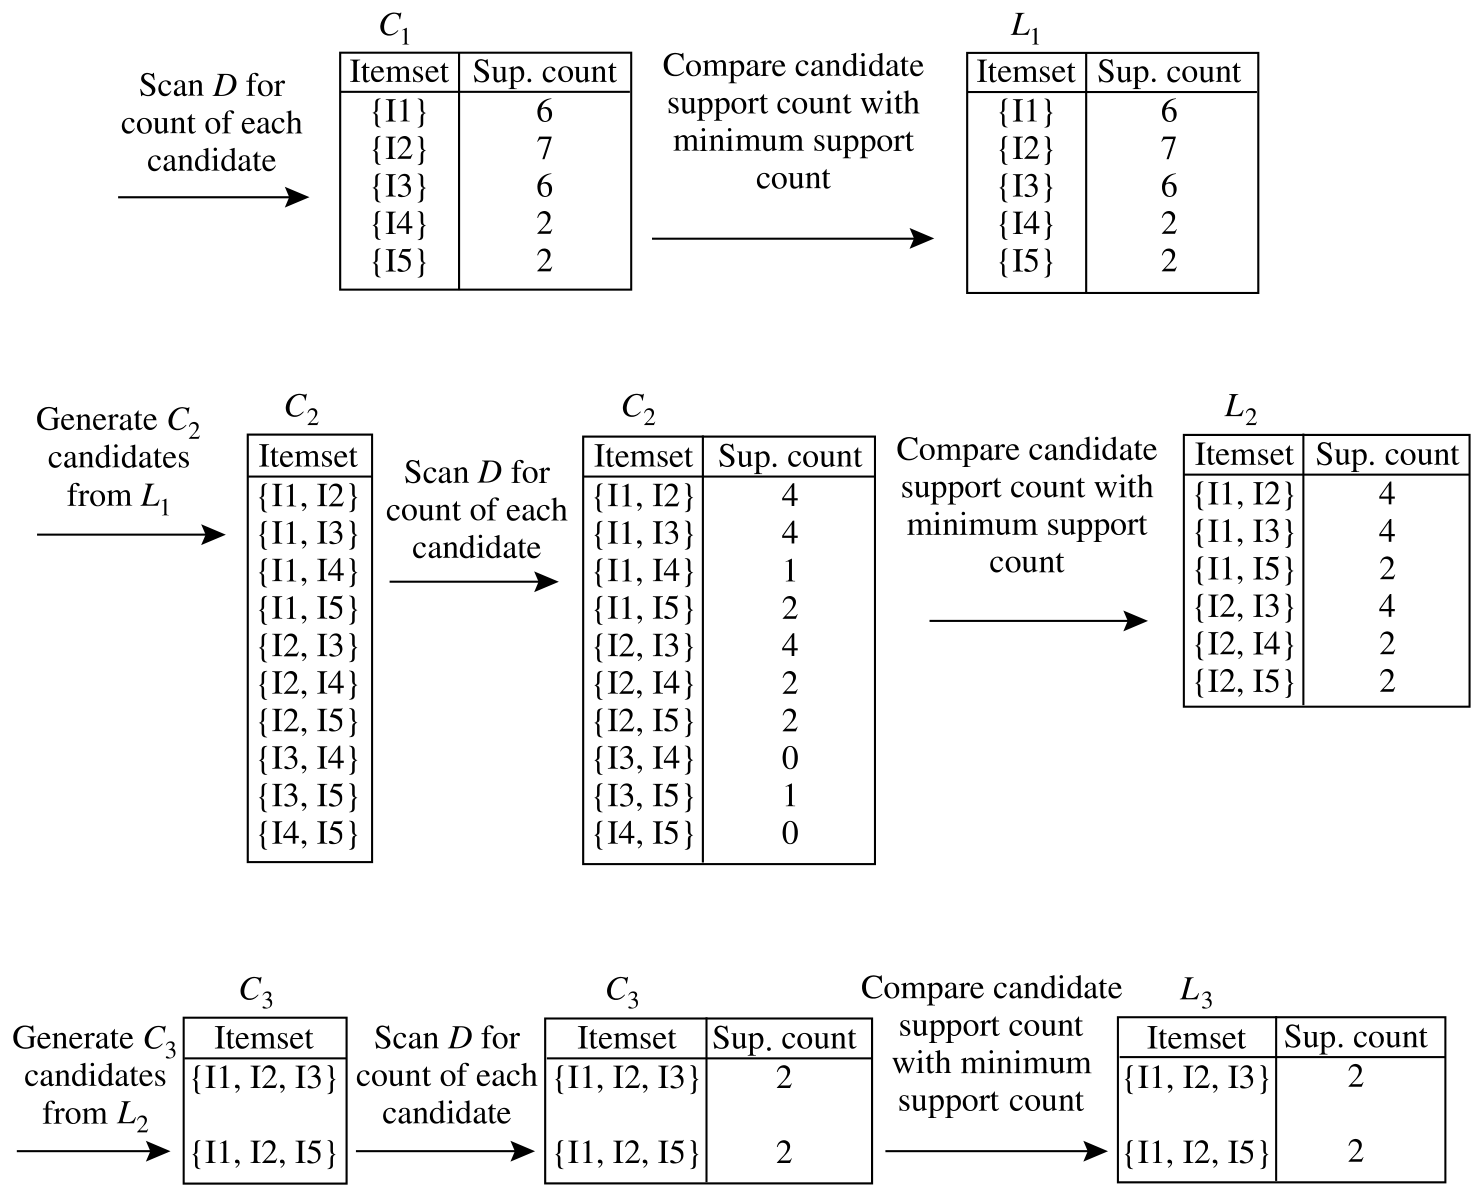
\includegraphics[width=\linewidth]{figs/c4_apriori_example.png}}{%
\lead{The level-wise run, drawn}
\begin{itemize}
  \item H\&K's 9-transaction example, min count 2: $C_1 \rightarrow L_1$, join to $C_2$,
    scan, $L_2$, join and \textbf{prune} to $C_3$, scan, $L_3$.
  \item Only 2 candidates survive into $C_3$: every other 3-itemset has an infrequent
    2-subset, so it is dropped \mk{without a scan}. That is the Apriori property at work.
  \item This is the shape every numerical in the companion writes out. H\&K Fig 6.2.
\end{itemize}}

\hr

\T{4.3 FP-Growth and the FP-Tree}

\Q{What is FP-Growth? Explain with example. How does it overcome Apriori's problems?}{\m{2+5}\m{8}\m{10}\m{2+6}}
{\color{sub}\footnotesize \tS{17} \yr{82 Bh, 81 Bh, 81 Ba, 80 Bh, 79 Bh, 79 Ba, 78 Bh, 75 Ch, 75 Ash, 74 Ch, 74 Ash, 73 Ch, 73 Shr, 72 Ka, 71 Shr, 70 Asa, 69 Ch}
\gap \mk{The single most-asked topic in this chapter.}}

\sbsr{0.52}{%
\lead{Key idea}
\begin{itemize}
  \item \mk{Generate NO candidates at all.}
  \item Compress $D$ into a \textbf{frequent-pattern tree (FP-tree)}, then mine that tree by
        \textbf{divide and conquer}.
  \item Only \mk{2 database scans} in total, against Apriori's $k+1$.
\end{itemize}
\lead{Step 1: build the FP-tree}
\begin{enumerate}
  \item \textbf{Scan 1}: count every item. Discard the infrequent ones.
  \item Sort the frequent items by \textbf{descending support} $\rightarrow$ the \textbf{F-list}.
        \mk{Break ties consistently} (alphabetically) and say so.
  \item \textbf{Scan 2}: for each transaction, keep only frequent items, \textbf{reorder them into
        F-list order}, and insert that path into the tree.
  \begin{itemize}
    \item Share a prefix with an existing path $\rightarrow$ just increment those counts.
    \item Otherwise create new nodes with count 1.
  \end{itemize}
  \item Maintain a \textbf{header table}: one entry per frequent item, with a \textbf{node-link}
        chain threading every occurrence of that item in the tree.
\end{enumerate}
\begin{itemize}
  \item \mk{Why descending order}: the most common items sit near the root, so paths share prefixes
        and the tree stays small.
\end{itemize}}{%
\lead{Step 2: mine the tree (FP-Growth)}
\begin{enumerate}
  \item Work \textbf{bottom-up} through the header table, ie \emph{least} frequent item first.
  \item For item $\alpha$, follow its node-links to collect its
        \textbf{conditional pattern base} $=$ every prefix path leading to $\alpha$,
        each carrying $\alpha$'s count at that node.
  \item Build the \textbf{conditional FP-tree} from that base, keeping only items that are still
        frequent \emph{within} it.
  \item \textbf{Recurse} on the conditional tree, concatenating $\alpha$ to each pattern found.
  \item If a conditional tree is a \textbf{single path}, just enumerate all subsets of that path.
\end{enumerate}
\mbox{}\hfill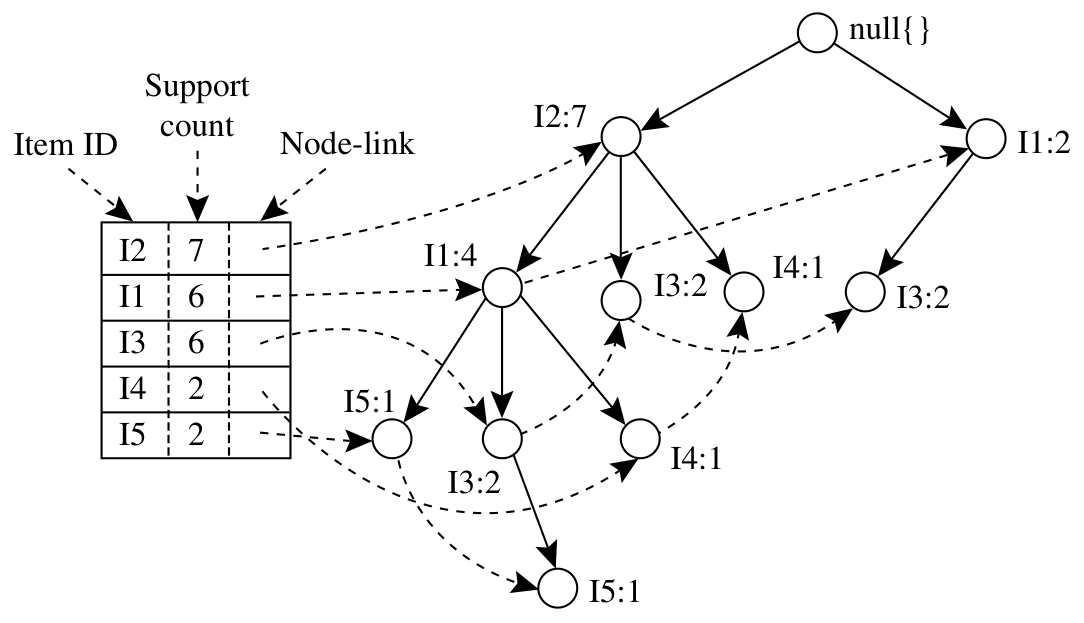
\includegraphics[width=0.62\linewidth]{figs/c4_fptree_hk.png}\hfill\mbox{}\par
{\color{sub}\scriptsize A finished FP-tree: \textbf{null} root, \texttt{item:count} nodes, and the
header table (item, support) whose dashed \textbf{node-links} thread every occurrence of an item.
Step 2 walks those links. H\&K Fig 6.7.}}

\penalty0\vspace{3pt}
\lead{Apriori vs FP-Growth \mk{(asked as a direct comparison 4 times)}}
\par
\begin{tabularx}{\textwidth}{@{}L{2.6cm}XX@{}}
\toprule
\hrow & \thead{Apriori} & \thead{FP-Growth} \\
Candidates & Generates them & \textbf{None} \\
DB scans & $k+1$ & \textbf{2} \\
Strategy & Breadth-first, level-wise & Depth-first, divide \& conquer \\
Structure & Hash tree & \textbf{FP-tree} (prefix tree) \\
Memory & Low & Tree must fit in memory \\
Speed & Slower & Roughly an order faster \\
\bottomrule
\end{tabularx}
\begin{itemize}
  \item \mk{FP-Growth's weakness}: if the tree does not fit in memory, or the data is very sparse
        so paths barely share prefixes, the advantage disappears.
\end{itemize}

\hr

\T{4.4 Handling Categorical Attributes}

\Q{How do you handle categorical attributes in data mining? Issues and fixes.}{\m{3+3}\m{2+3+3}\m{4}}
{\color{sub}\footnotesize \tP{3} \yr{79 Bh, 73 Shr, 72 Ch}}

\sbs{%
\lead{The problem}
\begin{itemize}
  \item Association analysis assumes \textbf{asymmetric binary} items (present / absent).
  \item Real tables hold categorical (Gender, Region) and continuous (Age, Income) attributes.
\end{itemize}
\lead{Handling: binarisation}
\begin{itemize}
  \item Convert each \textbf{(attribute, value) pair into one binary item}.
  \item Eg \texttt{Gender} $\rightarrow$ items \code{Gender=Male}, \code{Gender=Female}.
  \item Continuous attributes must be \textbf{discretised} first
        {\footnotesize$\rightarrow$ Ch 2, §2.2}, then binarised.
\end{itemize}}{%
\lead{Issues that arise \mk{(this is what 73 Shr wants)}}
\begin{itemize}
  \item \textbf{Too many items}: an attribute with many values explodes the item count.
        \mk{Fix}: group rare values into an ``Other'' category.
  \item \textbf{Many items are infrequent}: rare values never reach min\_sup, so patterns
        involving them are lost. \mk{Fix}: lower min\_sup, or use a per-item threshold.
  \item \textbf{Some items are far too frequent}: eg \code{Gender=Male} at $\approx$50\% produces
        masses of trivial redundant rules. \mk{Fix}: set a maximum support threshold too.
  \item \textbf{Redundancy}: values of one attribute are \textbf{mutually exclusive}, so an itemset
        containing \code{Gender=Male} \emph{and} \code{Gender=Female} has support 0 by construction.
        \mk{Fix}: never generate candidates that pair 2 values of the same attribute.
  \item \textbf{Loss of ordering} for ordinal attributes after binarisation.
\end{itemize}}

\hr

\T{4.5 Sequential, Subgraph and Infrequent Patterns}

\Q{Sequential patterns, subsequences, subgraph patterns}{\m{3+3}\m{2}\m{3}}
{\color{sub}\footnotesize \tF{5} \yr{79 Bh, 76 Ch, 76 Ash, 73 Ch, 72 Ka} \gap
\mk{Subsequence and subgraph enumeration are numericals} $\rightarrow$ companion.}

\sbsr{0.50}{%
\lead{Sequential patterns}
\begin{itemize}
  \item A \textbf{sequence} is an \emph{ordered} list of \textbf{elements}; each element is an
        unordered \emph{set} of items. \ $s = \langle e_1 e_2 \dots e_n\rangle$.
  \item \textbf{Length} $=$ number of \emph{items}; a \emph{$k$-sequence} has $k$ items.
        \mk{Not the number of elements} --- this is the usual mistake.
  \item \textbf{Subsequence}: $\langle a_1 \dots a_m\rangle$ is a subsequence of
        $\langle b_1 \dots b_n\rangle$ if there exist $i_1 < i_2 < \dots < i_m$ with
        $a_1 \subseteq b_{i_1},\ \dots,\ a_m \subseteq b_{i_m}$.
  \begin{itemize}
    \item \mk{Order across elements must be preserved; within an element it need not be.}
  \end{itemize}
  \item \textbf{Support} of a sequence $=$ fraction of data sequences containing it.
  \item \textbf{Algorithms}: \textbf{AprioriAll} \yr{76 Ash short note}, GSP, SPADE, PrefixSpan.
        AprioriAll applies the same anti-monotone pruning to sequences.
  \item \textbf{Uses}: web click-streams, purchase sequences over time, DNA, telephone call patterns.
\end{itemize}}{%
\lead{Subgraph patterns \yr{79 Bh \m{2}}}
\begin{itemize}
  \item Data $=$ a collection of \textbf{graphs} (molecules, web fragments, social networks).
  \item A \textbf{frequent subgraph} is one appearing in at least min\_sup of them.
  \item \textbf{Candidate generation by growing}, 2 schemes:
  \begin{itemize}
    \item \textbf{Vertex growing}: join 2 graphs sharing a common subgraph, add 1 vertex.
    \item \textbf{Edge growing}: join 2 graphs sharing a core, add 1 edge.
          \mk{Preferred} --- it generates fewer candidates.
  \end{itemize}
  \item \mk{The hard part is graph isomorphism}: deciding whether 2 drawings are the same graph.
        Handled with a canonical labelling.
  \item Algorithms: AGM, FSG, gSpan.
\end{itemize}
\lead{Infrequent / negative patterns}
\begin{itemize}
  \item A \textbf{negative pattern} is a set of items that appear together \emph{far less} often
        than independence would predict.
  \item Eg \code{\{Coke, Pepsi\}} --- customers buy one \emph{or} the other.
  \item Useful for detecting substitute products and for fraud (a combination that should
        never occur).
  \item \mk{Hard because} support is anti-monotone, so ``infrequent'' cannot be pruned the same way.
\end{itemize}}

\penalty0\vspace{3pt}
\sbsr{0.46}{%
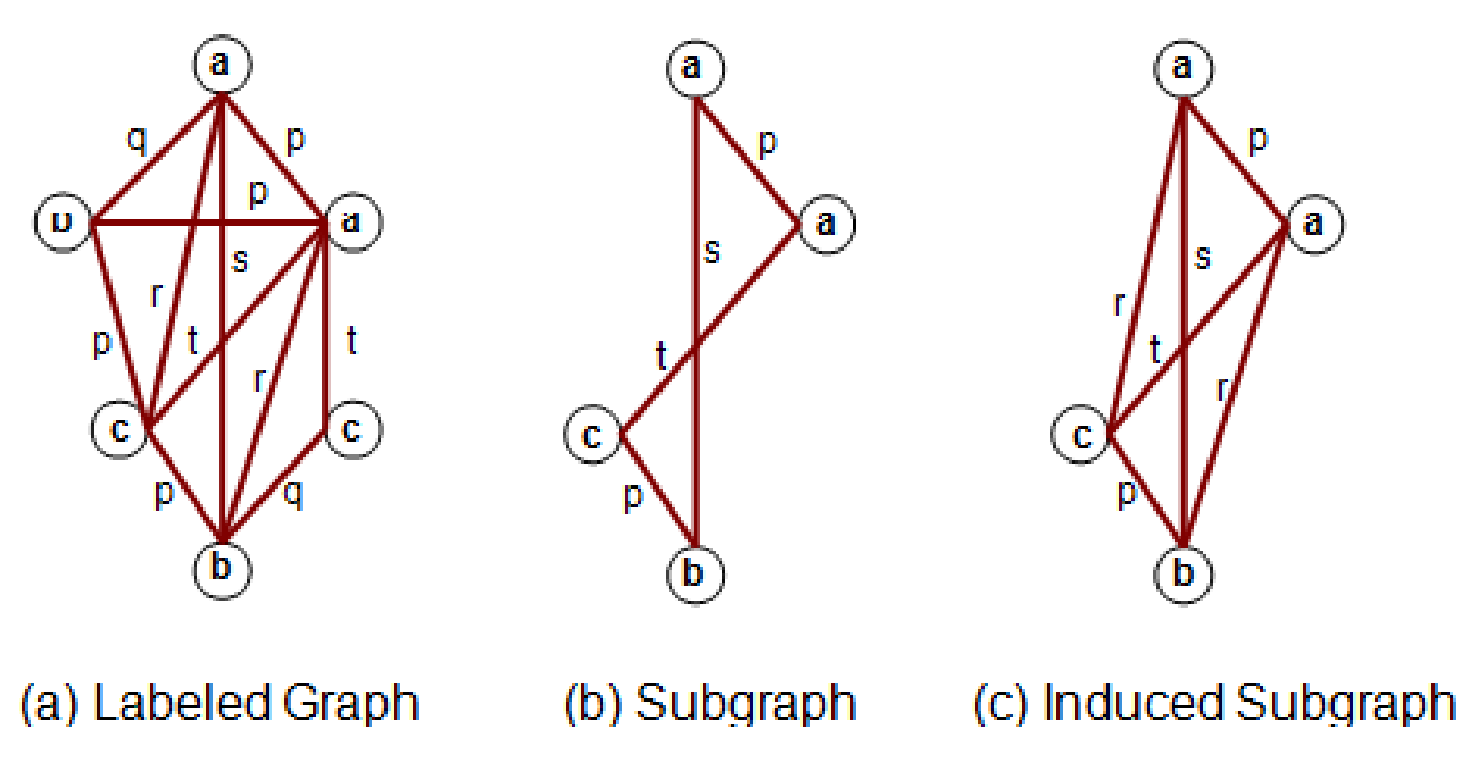
\includegraphics[width=\linewidth]{figs/c4_subgraph_types.png}}{%
\lead{Subgraph terms, drawn}
{\color{sub}\footnotesize (a) a labelled graph; (b) a \textbf{subgraph}: some of its vertices
and edges; (c) an \textbf{induced} subgraph: some vertices and \emph{every} edge between them.
Candidate generation grows these one vertex or one edge at a time. Mishra's Ch 4 notes, p9.}}

\hr

%-----------------------------------------------------------------------
\T{4.6 PYQ Mapping}

{\color{sub}\footnotesize \mk{N} $=$ solved in the Ch 4 Numerical companion.}

\creamq{4.1 Basics}{}
\begin{enumerate}
  \item \tS{7} Association analysis $+$ importance in market-basket analysis.
        \hfill \m{2+5} \yr{72 Ka} \m{10} \yr{72 Ch} \m{2+6} \yr{80 Ba}
  \item \tP{2} Why is association analysis required? $+$ Apriori principle w/ example.
        \hfill \m{2+6} \yr{75 Ash, 74 Ch}
  \item \tP{1} Importance of SUPPORT and CONFIDENCE $+$ FP-Growth w/ example. \hfill \m{10} \yr{72 Ch}
  \item \mk{N} \tP{1} Why is pattern evaluation important? $+$ statistical interestingness measures.
        \hfill \m{8} \yr{70 Ch}
  \item \tP{1} Why 100\% confidence is uninteresting but 99\% is. \hfill \m{4} \yr{80 Ba}
  \item \tP{1} Short note: Market Basket Analysis. \hfill \m{4} \yr{75 Ch}
\end{enumerate}

\creamq{4.2 Apriori}{}
\begin{enumerate}[start=7]
  \item \mk{N} Apriori, min support count 4, confidence 80\%, 7 transactions. \hfill \m{2+7} \yr{80 Bh}
  \item \mk{N} Candidate + large itemsets, min support 2. \hfill \m{4+5} \yr{80 Ba}
  \item \mk{N} Derive association rules, min sup 50\%, min conf 80\%. \hfill \m{8} \yr{79 Bh}
  \item \mk{N} Fast-food orders, min sup 2/9, min conf 7/9; frequent $k$-itemsets $+$ strong rules.
        \hfill \m{5+3} \yr{76 Ch}
  \item \mk{N} L-itemsets at $L=3$ w/ Apriori $+$ F-list w/ FP-Growth. \hfill \m{12} \yr{76 Ash}
  \item \mk{N} Candidate, frequent itemsets and rules, min sup 20\%, min conf 80\%. \hfill \m{8} \yr{74 Ash}
  \item \mk{N} Apriori w/ support 50\%. \hfill \m{10} \yr{70 Ch}
  \item \tP{1} How does Apriori optimise the brute-force approach? \hfill \m{10} \yr{71 Ch}
  \item \tP{1} What are association rules? How does Apriori generate them? \hfill \m{10} \yr{71 Shr}
\end{enumerate}

\creamq{4.3 FP-Growth}{}
\begin{enumerate}[start=16]
  \item \tS{7} What is FP-Growth? Explain w/ example.
        \hfill \m{2+5} \yr{80 Bh} \m{8} \yr{74 Ash} \m{10} \yr{71 Shr} \m{2+6} \yr{75 Ash}
        \m{1+8} \yr{72 Ka} \m{2+5} \yr{81 Ba}
  \item \mk{N} Draw FP-tree for the given 5-transaction table. \hfill \m{4+4} \yr{75 Ch}
  \item \mk{N} Limitation of Apriori vs FP-Growth $+$ \code{\{M,O,N,K,E,Y\}} database,
        min sup 60\%, min conf 80\%. \hfill \m{2+7} \yr{81 Ba}
  \item \mk{N} Build FP-tree transaction by transaction $+$ mine it, threshold 33.34\% / 60\%.
        \hfill \m{4+4} \yr{78 Bh}
  \item \mk{N} How does FP-Growth overcome Apriori? $+$ generate the FP-tree. \hfill \m{2+8} \yr{74 Ch}
  \item \mk{N} FP-tree $+$ association rules, support 30\%, confidence 75\%. \hfill \m{10} \yr{73 Shr}
  \item \tP{1} Short note: FP-Tree. \hfill \m{5} \yr{79 Bh}
\end{enumerate}

\creamq{4.4 / 4.5 Categorical, Sequential, Subgraph}{}
\begin{enumerate}[start=23]
  \item \mk{N} Handle categorical attributes $+$ generate 4 subsequences from
        $\langle\{2,3,5\},\{6,7,8\},\{9,1\},\{7,4\}\rangle$. \hfill \m{3+3} \yr{79 Bh}
  \item \tP{1} Categorical data, issues, how to handle them. \hfill \m{2+3+3} \yr{73 Shr}
  \item \mk{N} List all 4-subsequences of $\langle\{1,3\}\{2\}\{2,3\}\{4\}\rangle$ $+$ draw
        candidate subgraphs by edge growing. \hfill \m{3+3} \yr{76 Ch}
  \item \tP{1} What are subgraph patterns? \hfill \m{2} \yr{79 Bh}
  \item \tP{3} Short notes: AprioriAll \yr{76 Ash} $\cdot$ Sequential pattern \yr{72 Ka} $\cdot$
        Categorical data \yr{72 Ch}. \hfill \m{3}\m{4}
\end{enumerate}

\creamq{Papers added by the 2026-09 merge}{}
{\color{sub}\footnotesize The six papers of \code{DM4.1BCT.pdf} (2082 Bh, 2081 Bh, 2079 Ba, 2073 Ch, 2070 Asa, 2069 Ch), indexed here for the
first time --- the notes were built before that scan was merged. \mk{N} $=$ solved in this chapter's companion. \added}
\begin{itemize}
  \item \mk{N} Support and confidence $+$ derive rules, min sup 60\%, min conf 80\%, 5 transactions. \hfill \m{2+8} \yr{82 Bh}
  \item \mk{N} Apriori with \mk{confidence 65\%} and min support 50\%, 4 transactions. \hfill \m{2+6} \yr{81 Bh}
  \item \mk{N} Apriori on a $7\times9$ \textbf{binary} table (min\_sup 20\%) $+$ \mk{can any rule exist at any confidence threshold?} \hfill \m{5+3} \yr{79 Ba} \added
  \item \mk{N} Apriori in market-basket analysis, both thresholds 50\%. \hfill \m{3+7} \yr{73 Ch}
  \item Advantages of FP-Growth over Apriori $+$ FP-Growth w/ example. \hfill \m{2+6} \yr{81 Bh}
  \item How does FP-Growth generate frequent itemsets \textbf{without candidate generation}? \hfill \m{6} \yr{79 Ba}
  \item Use of FP-Growth in market-basket analysis \yr{73 Ch} $\cdot$ FP-Growth in detail \yr{70 Asa}. \hfill \m{10}\m{12}
  \item What is frequent itemset mining? How do Apriori \emph{and} FP-Growth optimise the brute-force approach? \hfill \m{15} \yr{69 Ch}
  \item How can Apriori be used to find rules \emph{out of} a frequent itemset? \hfill \m{7} \yr{69 Ch}
  \item Association rules $+$ their importance w/ example \yr{70 Asa} $\cdot$ short note \textbf{FP Growth} \yr{82 Bh}. \hfill \m{6}\m{5}
  \item Sequential pattern and sub-graph pattern w/ suitable example. \hfill \m{4+4} \yr{73 Ch}
\end{itemize}

\lead{Coverage check}
\begin{itemize}
  \item All Ch 4 PYQs covered. \textbf{14 are numerical} $\rightarrow$ companion.
  \item \textbf{Gaps filled by research} \added:
  \begin{itemize}
    \item The \textbf{null-invariant measures} (all\_conf, max\_conf, Kulc, cosine) and the
          game/video counter-example for \yr{70 Ch}: your notes define only support and confidence.
    \item \textbf{Issues with categorical attributes} \yr{73 Shr}: the mutual-exclusion and
          too-frequent-item problems are in no source note.
    \item \textbf{Edge vs vertex growing} for subgraphs.
  \end{itemize}
\end{itemize}

\lead{Sources used for this chapter}
\begin{itemize}
  \item \textbf{Han \& Kamber 3rd ed} ch 6 (frequent patterns, Apriori, FP-Growth, pattern
        evaluation) and ch 7 (advanced pattern mining). \mk{Primary authority.}
  \item \textbf{DBK Lectures 12--14}, \code{data mining\_/Chapter-4 Association Analysis.pdf},
        \code{Associations\_Rule\_mining.ppt}, \code{FP-Growth algorithm.ppt},
        \code{FP Tree.pdf}, \code{Episode\_Mining.PDF}.
\end{itemize}
